
\chapter{Introduction}
\label{Chap:Intro}
This thesis considers the problem of tracking human wrist movements during free living.
These movements would need to be tracked cintinuously all day,
storing the data so that it can be processed later.
To capture this information we need an accekerometer and a gyroscope.
Accelerometers typically draw a current of 270$\mu$,
while a gyroscope can consume 3 - 10$\mu$ of current.
These devices are powered by a battery,
and common small batteries used in wrist based devices have a capacity of 20 - 200mAh.
These capacities allow for an accelerometer based device to operate up to a week,
however, depending on the size of the battery,
devices with a gyroscope typically operate for a couple of hours because of their higher current consumption.
The battery size also affects the size of the device as the battery is usually the largest part in the device.
Since we want our device to be mounted on the wrist,
we would like our battery size to be small enough to be comfortably worn on the wrist.

Our group is motivated by the vision of a wrist mounted device that can track wrist motion activity and
detect when a person is eating,
and also be able to count the number of bites in each meal.
In previous research we have demonstrated algorithms where periods of eating can be detected with 81\% accuracy,
and the number of bites in these meals can be detected with 86\% accuracy.
To further this research,
we reqyure a device that will allow us to record wrist motion data for a period of days to weeks and can be used across a large number of subjects.
Due to this extended interval of use,
the device needs a long battery life,
and has to be comfortable to wear.


\section{Motivation}
\label{Sec:Motivation}

 CDC (Centers for Disease Control and Prevention) reports mention one
 \textemdash{} third of the adult American population as 
 obese, while sixty nine percent of the population is considered 
 overweight. The agency defines individuals with a Body Mass
 Index of twenty five and above as overweight~\cite{ogden2010prevalence}.
 This number is rising in children too, with eighteen
 percent children between the ages of 12 \textemdash{} 18
 years considered obese. When a group
 of individuals was asked to count the number of bites taken over
 a 24 hour period, 40\% lost count or forgot the count entirely~\cite{mahoney1975obese}.

Our group is motivated by the vision of a wrist-worn device that can continuously
track wrist motion to detect when a person is eating, and to count the number
of bites consumed during each eating activity.  The group has previously demonstrated
algorithms that achieve 81\% accuracy for detecting eating activities during all-day
wrist motion tracking \cite{dong2013detecting}, and for counting bites with 86\% accuracy during meals \cite{dong2012new}.
To improve these techniques, we require a device that allows us to collect data from
a large number of subjects over a period of days to weeks. Thus, we require a device that is
comfortable to wear, will operate for an entire day on a single battery charge, and
has a relatively low cost.
 
\section{Wrist Based Activity Monitors}
\label{Sec:FitnessTracking}
With the increase in smart phone sales,
we see a huge rise in devices that help track our daily activities.
Fitness trackers in the market currently offer a range of services. The Fitbit \cite{Web:FitBitOfficial},\cite{Web:FitbitFlex} and Jawbone \cite{Web:JawBoneWebsite} series of sensors allow for exercise and sleep monitoring using wrist movements. This data is then synchronized with a computer or a mobile phone, and can be viewed graphically by the user. Another consumer electronic segment that has now emerged is smart watches. These watches contain electronic components that make them functionally similar to a mobile phone, and are small enough to wear on the wrist. They contain low power displays and have a host of power saving techniques to have a long battery life. Table \ref{Tab:IntroComp} shows a list of select devices on the market that can track wrist motion and could potentially be used for the bite counting applicaiton.
\inputfile{IntroCompTable.tex}
As we can see, most of the wearable devices in the market are limited to counting the number of calories expended and thus not many options exist for counting the number of calories consumed. Most of the options available are not optimized for recording wrist movement data for an entire day.
The iPhone, which would work as expected is not suitable as a wrist mounted device, and the SHIMMER has a high procurement cost for development.
\begin{figure}
\begin{center}
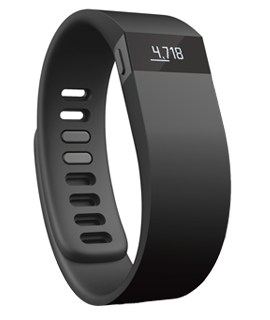
\includegraphics[width=0.4\textwidth]{images/JawFit.png}
\caption{The Fitbit flex activity tracker \cite{Web:FitbitImage}}
\label{fig:FitbitJawbone}
\end{center}
\end{figure}

\section{Previous Work}
Our group has been involved with bite counting by tracking wrist motion for half a decade.
Initial research~\cite{dong2012new} worked on identifying if this was a feasible idea.
During the early stages,
sensors were mounted directly on the wrist,
and a cable connected the sensor to a personal computer.
The computer would log data from the sensors and identify when the user took a bite of food.
Needless to say,
mobility by the user was limited,
and they would have to consume all of their meal within range of the computer cable.
Later work switched to a device that could process this information from the sensor in real time,
and predict the total number of bites taken by the user in a meal.
This device was able to store only the number of bites, 
but not the actual data captured from the sensors.
It was widely reviewed and reported by the media.
Figure \ref{Fig:BCEater} shows a photograph from the research groups website showing the final device which was mass manufactured.

\begin{figure}
        \centering
        % \begin{subfigure}[b]{0.3\textwidth}
                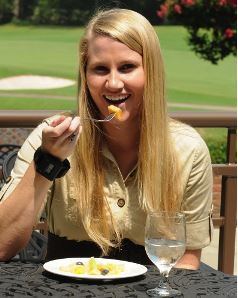
\includegraphics[]{images/BCEater.JPG}

                \label{fig:gull}
        % \end{subfigure}%
        ~ %add desired spacing between images, e. g. ~, \quad, \qquad, \hfill etc.
          %(or a blank line to force the subfigure onto a new line)
        % \begin{subfigure}[b]{0.3\textwidth}
        %         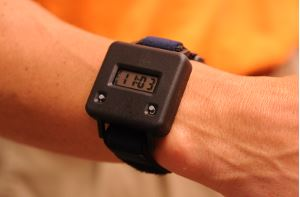
\includegraphics[width=\textwidth]{images/BCWrist.JPG}
        %         \caption{Close up photo of the bite counter mounted on a wrist.}
        %         \label{fig:tiger}
        % \end{subfigure}
         \caption{Photograph of a person using the Bite Counter while eating.}\label{Fig:BCEater}
\end{figure}

\section{Wearable Wrist Motion Tracker}
\label{Sec:WearbleTracker}
\begin{figure}
\begin{center}
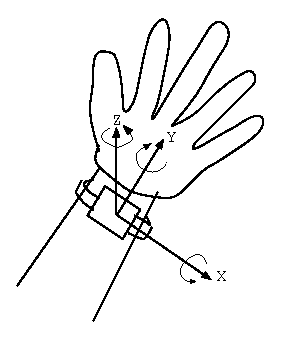
\includegraphics{images/HandAxis.eps}
\caption{A wrist watch shaped device showing the different axis being recorded.}
\label{fig:HandAxis}
\end{center}
\end{figure}
Earlier work by the group showed a device that is capable of
detecting bites by monitoring wrist movement~\cite{drennan2010assessment}.
We are motivated by the problem of monitoring calorie consumption by
creating a wrist watch like device that is specifically designed
to for the function of tracking and storing wrist motion data all day
on a single battery. Our goal for this device is to improve on the
battery life, programmability and the cost of procurement compared to
the devices seen in table \ref{Tab:IntroComp}
